\documentclass[11pt]{article}

\usepackage[T1]{fontenc}
\usepackage[utf8]{inputenc}
\usepackage[english]{babel}
\usepackage{xspace}
\usepackage{parskip}
\usepackage{amsmath}
\usepackage{amsfonts}
\usepackage{amssymb}
\usepackage{enumitem}
\usepackage[dvipsnames]{xcolor}
\usepackage{graphicx}
\usepackage{subcaption}
\usepackage{booktabs}
\usepackage{float}
\usepackage{array}
\usepackage[
    paper = a4paper,
    margin = 2.5cm,
    top = 2cm,
    bottom = 2cm
]{geometry}
\usepackage[colorlinks = true]{hyperref}


%%%%%%%%%%%%%%%%%%%%%%%%%%%%%%%%%%%%%%%%%%%%%%%%%%%%%

\newcommand{\iLaTeX}{i\LaTeX{}\xspace}

\title{A test file for \iLaTeX}
\author{Camille Gobert (\url{camille.gobert@ens.fr})}
\date{\today}

\linespread{1.05}


%%%%%%%%%%%%%%%%%%%%%%%%%%%%%%%%%%%%%%%%%%%%%%%%%%%%%

% You can view the result on Overleaf:
% https://www.overleaf.com/read/cvhwtykfnzpn

\begin{document}
    % Title
    \maketitle
    
    % Body
    Lorem ipsum dolor sit amet.
    Text \emph{accentu\'e} should be supported.
    
    \textbf{This is bold text.}
    \textit{This is italic text.}
    
    This is a \href{https://www.lri.fr/}{hyperlink} to LRI's website.
    
    % Example of some maths
    \paragraph{}
    Inline maths such as $x^2$ are supported, as well as 
    $$e^{i\pi} + 1 = 0$$
    
    % Example of a table
    \begin{table}[h]
        \centering
        \begin{tabular}{rl}
            \toprule
            \textbf{Symbol} & \textbf{Value} \\
            \midrule
            $x$ & 1 \\
            $y$ & 2 \\
            $z$ & 3 \\
            \bottomrule
        \end{tabular}
        \caption{Random table.}
        \label{tab:random}
    \end{table}
    
    % Example of a figure
    \begin{figure}[h]
    \href{{custom://some-invalid-uri/12345#abc?def=ghi}}{%
        \parbox{\textwidth}{
            \centering
            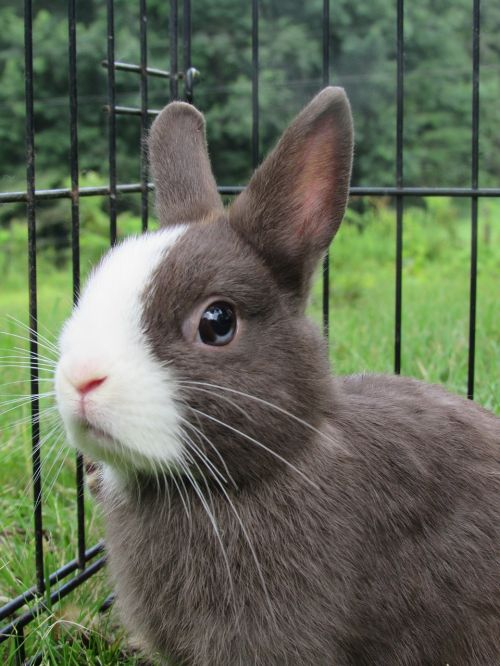
\includegraphics[width=201px, trim=0px 40px 38px 0px, clip]{img/rabbit.jpg}
            \caption{Picture of a rabbit.}
            \label{fig:rabbit}
        }
    }
    \end{figure}
    
    % Bibliography
    \bibliographystyle{plain}
    \bibliography{refs}
\end{document}
